\chapter{Introduction}
\label{chapter:introduction}

\newenvironment{introduction2}
{\quote\itshape}
{\endquote}

\begin{introduction2}
\end{introduction2}

\section{Context and Motivation}
In recent years, there has been an alarming increase in firearm-related crime. In 2022, the Federal Bureau of 
Investigation reported fifty active shooter incidents in the \ac{us}. These were spread across 25 states, 
and 313 casualties in these incidents, 
Figure \ref{fig:casualties}, including 100 deaths and 213 injuries, with the most severe incident causing seven 
fatalities and 48 injuries \selectlanguage{english}\cite{rfc37}.

Notably, there was a 18\% decrease in such incidents in 2021 but a significant 66.7\% increase compared to 2018, as shown in Figure \ref{fig:incidents}.

\begin{figure}[h]
    \centering
    \begin{minipage}{0.42\textwidth}
        \centering
        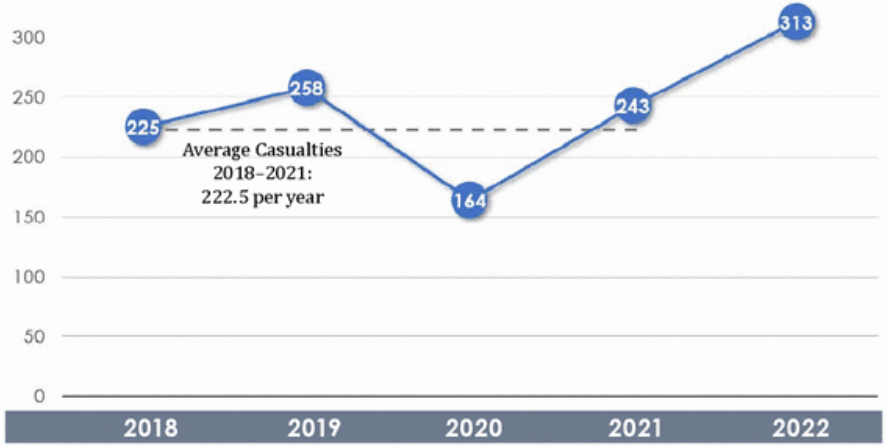
\includegraphics[width=1\linewidth]{figs/active-shooter-incidents.png}
        \caption{Active shooter incidents casualties in the \ac{us} \selectlanguage{english}\cite{rfc37}}
        \label{fig:casualties}
    \end{minipage}\hfill
    \begin{minipage}{0.45\textwidth}
        \centering
        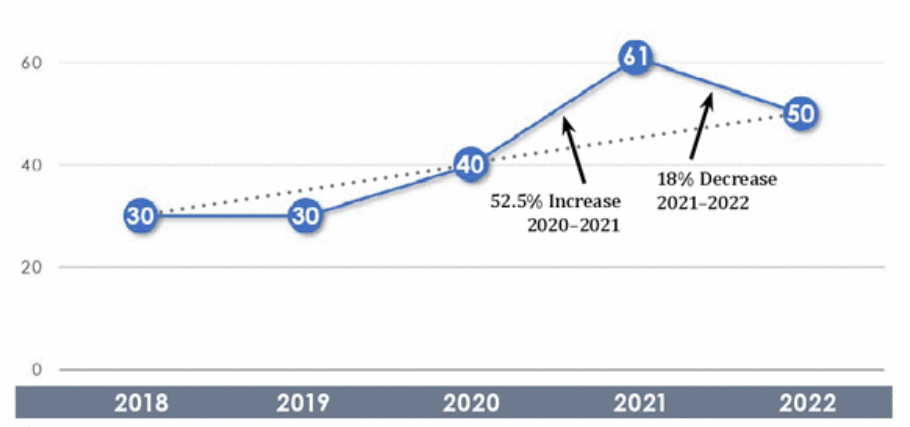
\includegraphics[width=1\linewidth]{figs/active-shooter-us.png}
        \caption{Active shooter incidents in the \ac{us} \selectlanguage{english}\cite{rfc37}}
        \label{fig:incidents}
    \end{minipage}
\end{figure}

Despite the existence of strict gun laws in numerous countries, the accessibility of firearms remains relatively 
high. The \ac{us} is the global leader in civilian gun ownership, with an estimated 120.5 firearms per 100 
people, which is nearly twice as high as the country with the second-highest rate.

Despite the existence of strict gun laws in many countries, firearm access remains relatively 
easy \selectlanguage{english}\cite{rfc39, rfc40}. The \ac{us} is the global leader in civilian gun 
ownership, with an estimated 120.5 firearms per 100 
people, which is nearly twice as high as the country with the second-highest rate.
\selectlanguage{english}\cite{rfc32}.

Within the 50 active shooter incidents in 2022, a total of 61 firearms were utilized, as shown in Figure \ref{fig:fbi-firearms}. Handguns were the most frequently used, accounting for 29 of the weapons, followed closely by rifles at 26.

\begin{figure}[h]
    \centering 
    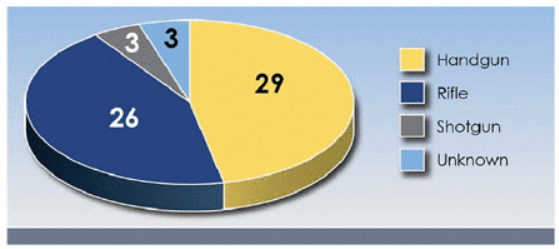
\includegraphics[width=0.4\textwidth]{figs/firearms.png} 
    \caption{Firearm used by active shooters in the \ac{us} \selectlanguage{english}\cite{rfc37}}
    \label{fig:fbi-firearms}
\end{figure}

In relation to Portugal, as RASI  \selectlanguage{english}\cite{rfc41}, reports, there has been a substantial 
increase in criminal activity. The total number of general crime reports registered 
by the Public Security Forces was 343845 in 2022, which is an increase of 42451 compared to 2021, 
representing a 14.1\% rise. Specifically, the total number of reported violent and serious crimes was 
13281, up by 1667 from the previous year, marking a 14.4\% increase, as shown in Figure \ref{fig:crimes-portugal}.

\begin{figure}[h]
    \centering 
    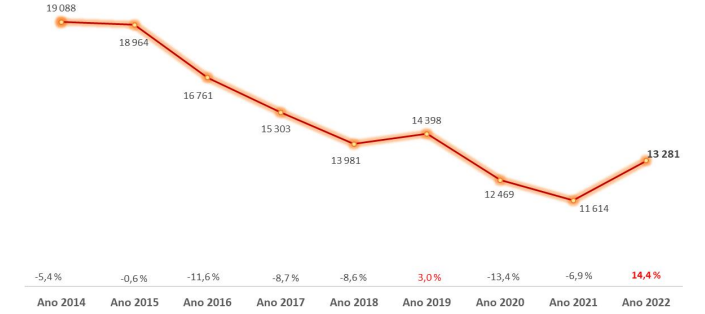
\includegraphics[width=0.8\textwidth]{figs/crimes-portugal.png} 
    \caption{Crime Rates in Portugal from 2014 to 2022 \selectlanguage{english}\cite{rfc41}}
    \label{fig:crimes-portugal}
\end{figure}

Figure \ref{fig:geo-crimes} shows a geographically decrease in the districts of Braga (-5.1\%), Bragança (-17.9\%), and Vila Real (-10\%). Conversely, there was a significant increase in Lisbon (+11.4\%), Porto (+11.3\%), Faro (+23.9\%), and the Autonomous Region of Madeira (+52\%).

\begin{figure}[h]
    \centering 
    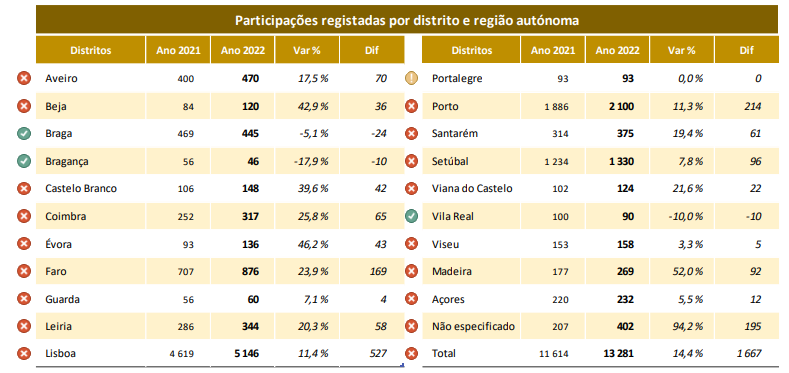
\includegraphics[width=0.75\textwidth]{figs/geo-crimes-rate.png} 
    \caption{Geographical Distribution of Crime Rate Increase in Portugal by District in 2022 \selectlanguage{english}\cite{rfc41}}
    \label{fig:geo-crimes}
\end{figure}

Along the years, It was noticed that \ac{cctv} systems have became a 
crucial tool for crime prevention. Research indicates a 
correlation between \ac{cctv} deployment and a reduction in crime rates, especially in car parks 
\selectlanguage{english}\cite{rfc33}. For example, in Florida, the implementation of \ac{cctv} has resulted in 
crime rate reductions of up to 51\% in certain areas \selectlanguage{english}\cite{rfc34}. Alongside its growing 
popularity worldwide, \ac{cctv} surveillance has generated debates concerning its effectiveness, efficiency, and 
related privacy issues. Critics of \ac{cctv} surveillance frequently raise concerns about the invasion of privacy 
and the risk of violating privacy laws \selectlanguage{english}\cite{rfc38}.

A significant challenge in operating \ac{cctv} systems is the reliance on human monitoring, which is susceptible to errors due to fatigue or distraction. Additionally, the financial implications of \ac{cctv}, including the costs associated with constructing and maintaining these surveillance systems, form an essential part of the discussion. These costs must be weighed against the potential benefits in crime reduction and public safety \selectlanguage{english}\cite{rfc38}. 

The effectiveness of \ac{cctv} in controlling crime varies and is influenced by several factors, including geographic location, crime types, and the strategies employed for camera monitoring. Studies have revealed that \ac{cctv} operations managed by private security personnel tend to have a more substantial crime prevention impact compared to those overseen by police \selectlanguage{english}\cite{rfc36}. In Sweden's deprived neighborhoods, the use of \ac{cctv} has led to a decrease in violent crimes, though it has not significantly affected property crime rates or the clearance of crimes \selectlanguage{english}\cite{rfc35}.

\ac{cctv} systems have emerged as key tools in crime prevention, offering the ability to reduce specific types of crime, especially in environments where they are actively monitored and used alongside other interventions \selectlanguage{english}\cite{rfc35}. 
\section{Objectives}
The primary goal of this project is to advance in the field of public safety and security through the development of a Deep Learning-Based system for real-time weapon detection in \ac{cctv} surveillance footage, designed for the detection and classification of weapons, such as firearms and knives. This includes several key aspects:
\begin{itemize}
    \item Exploration of Current Technologies and Methods: thorough review of the state-of-the-art technologies and methodologies used in real-time, analyzing existing approaches' effectiveness, efficiency, and applicability in various real-world scenarios;
    \item Identification and Analysis of Public Databases: identify public databases that contain relevant data on anomalous objects;
    \item Development of a Deep Learning Model: develop a state-of-the-art deep learning model capable of accurately identifying and classifying firearms or knives in diverse and challenging surveillance scenarios;
    \item Architecture Design and Prototyping: proposing and developing a prototype solution with a well-defined architecture;
    \item Performance Evaluation and Limitation Analysis: extensive testing of the prototype in various real-life scenarios to evaluate its performance, accuracy, and reliability;
\end{itemize}

The expectation is that the application and model developed through this research will surpass existing solutions in terms of efficiency, accuracy, and practicality. To achieve this, it is imperative to conduct a comprehensive analysis of the work done by other researchers. This examination will not only provide insights into the most effective strategies and methodologies but will also shed light on the common challenges and barriers encountered in similar attempts.  
\section{Outline of the Document}
The document is organized into subsequent chapters as follows: 

\begin{itemize}
    \item Chapter 2 offers a detailed analysis of the 
    existing research and technologies in weapon detection, focusing on critical aspects like weapon categorization, 
    the significance of \ac{cctv}, and the application of deep learning algorithms;
    \item Chapter 3 discusses the high-level architecture of the project and details the work plan, including 
    milestones and a Gantt chart to illustrate the project timeline;
    \item Chapter 4 describes the implementation of the application, including the system architecture and a 
    comprehensive examination of each component involved in the development process;
    \item Chapter 5 presents the tests conducted and the results obtained, providing a thorough analysis of 
    the performance and accuracy of the implemented system;
    \item Chapter 6 concludes the thesis by summarizing the key findings, discussing the implications of the 
    results, and suggesting directions for future work in the field of weapon detection.
\end{itemize}